\documentclass[12pt]{beamer}
\usepackage{../Estilos/BeamerMAF}
\usepackage{../Estilos/ColoresLatex}
\usetheme{Warsaw}
\usecolortheme{seahorse}
%\useoutertheme{default}
\setbeamercovered{invisible}
% or whatever (possibly just delete it)
\setbeamertemplate{section in toc}[sections numbered]
\setbeamertemplate{subsection in toc}[subsections numbered]
\setbeamertemplate{subsection in toc}{\leavevmode\leftskip=3.2em\rlap{\hskip-2em\inserttocsectionnumber.\inserttocsubsectionnumber}\inserttocsubsection\par}
\setbeamercolor{section in toc}{fg=blue}
\setbeamercolor{subsection in toc}{fg=blue}
\setbeamercolor{frametitle}{fg=blue}
\setbeamertemplate{caption}[numbered]

\setbeamertemplate{footline}
\beamertemplatenavigationsymbolsempty
\setbeamertemplate{headline}{}


\makeatletter
\setbeamercolor{section in foot}{bg=gray!30, fg=black!90!orange}
\setbeamercolor{subsection in foot}{bg=blue!30}
\setbeamercolor{date in foot}{bg=black}
\setbeamertemplate{footline}
{
  \leavevmode%
  \hbox{%
  \begin{beamercolorbox}[wd=.333333\paperwidth,ht=2.25ex,dp=1ex,center]{section in foot}%
    \usebeamerfont{section in foot} \insertsection
  \end{beamercolorbox}%
  \begin{beamercolorbox}[wd=.333333\paperwidth,ht=2.25ex,dp=1ex,center]{subsection in foot}%
    \usebeamerfont{subsection in foot}  \insertsubsection
  \end{beamercolorbox}%
  \begin{beamercolorbox}[wd=.333333\paperwidth,ht=2.25ex,dp=1ex,right]{date in head/foot}%
    \usebeamerfont{date in head/foot} \insertshortdate{} \hspace*{2em}
    \insertframenumber{} / \inserttotalframenumber \hspace*{2ex} 
  \end{beamercolorbox}}%
  \vskip0pt%
}
\makeatother

\makeatletter
\patchcmd{\beamer@sectionintoc}{\vskip1.5em}{\vskip0.8em}{}{}
\makeatother

\newlength{\depthofsumsign}
\setlength{\depthofsumsign}{\depthof{$\sum$}}
\newcommand{\nsum}[1][1.4]{% only for \displaystyle
    \mathop{%
        \raisebox
            {-#1\depthofsumsign+1\depthofsumsign}
            {\scalebox
                {#1}
                {$\displaystyle\sum$}%
            }
    }
}
\def\scaleint#1{\vcenter{\hbox{\scaleto[3ex]{\displaystyle\int}{#1}}}}
\def\scaleoint#1{\vcenter{\hbox{\scaleto[3ex]{\displaystyle\oint}{#1}}}}
\def\bs{\mkern-12mu}


\title{\large{Funciones Gamma y Beta}}
\subtitle{Tema 1 - La física y la geometría}

\author{M. en C. Gustavo Contreras Mayén}
\makeatletter

\setbeamertemplate{footline}
{
  \leavevmode%
  \hbox{%
  \begin{beamercolorbox}[wd=.333333\paperwidth,ht=2.25ex,dp=1ex,center]{section in foot}%
    \usebeamerfont{section in foot} \insertsection
  \end{beamercolorbox}%
  \begin{beamercolorbox}[wd=.333333\paperwidth,ht=2.25ex,dp=1ex,center]{subsection in foot}%
    \usebeamerfont{subsection in foot}  \insertsubsection
  \end{beamercolorbox}%
  \begin{beamercolorbox}[wd=.333333\paperwidth,ht=2.25ex,dp=1ex,right]{date in head/foot}%
    \usebeamerfont{date in head/foot} {T1 - Cuarta presentación} \hspace*{2em}
    \insertframenumber{} / \inserttotalframenumber \hspace*{2ex} 
  \end{beamercolorbox}}%
  \vskip0pt%
}
\makeatother
\date{}

\begin{document}
\maketitle
\fontsize{14}{14}\selectfont
\spanishdecimal{.}

\section*{Contenido}
\frame[allowframebreaks]{\tableofcontents[currentsection, hideallsubsections]}

\section{Integrales como funciones.}
\frame{\tableofcontents[currentsection, hideothersubsections]}
\subsection{Funciones de apoyo}

\begin{frame}
\frametitle{Integrales como funciones}
Las integrales son uno de los medios matemáticos más convenientes con los que se pueden definir nuevas funciones.
\\
\bigskip
\pause
Si el integrando o los límites de integración incluyen parámetros, esos parámetros pueden tratarse como variables y la integral misma como una función de esos parámetros.
\end{frame}
\begin{frame}
\frametitle{Integrales como funciones}
Haremos una revisión de algunas funciones más importantes que normalmente se definen en términos de integrales.
\end{frame}

\subsection*{La función Gamma}

\begin{frame}
\frametitle{De la función Gamma}
La función Gamma $\Gamma (x)$ aparece ocasionalmente en problemas de física tales como:
\pause
\setbeamercolor{item projected}{bg=capri,fg=black}
\setbeamertemplate{enumerate items}{%
\usebeamercolor[bg]{item projected}%
\raisebox{1.5pt}{\colorbox{bg}{\color{fg}\footnotesize\insertenumlabel}}%
}
\begin{enumerate}[<+->]
\item Cálculo de probabilidades en mecánica estadística.
\item La normalización de las funciones de onda para el potencial de Coulomb en mecánica cuántica.
\end{enumerate}
\end{frame}
\begin{frame}
\frametitle{Su uso en la física}
En realidad la función $\Gamma (x)$ tiene pocas aplicaciones directas en física, \pause sin embargo es importante porque nos permite desarrollar otras funciones que si tienen una aplicación directa en la física, como por ejemplo: las funciones de Bessel.
\end{frame}
\begin{frame}
\frametitle{Relación entre las funciones de apoyp}
La relación entre las funciones $\Gamma (x)$ y $B (x, y)$ también nos permitirán expresar de manera más compacta los resultados que se obtendrán al resolver ciertas ecuaciones diferenciales que veremos a lo largo del curso.
\end{frame}
\begin{frame}
\frametitle{Necesidad en el manejo de éstas funciones}
Es por ello que al manejar debidamente estas funciones (y sus variantes), tendremos más herramientas para nuestro objetivo: \pause resolver un problema de la física mediante el uso de funciones especiales, y con ello, interpretar el fenómeno que estudiamos.
\end{frame}
\begin{frame}
\frametitle{Punto importante}
Para el manejo de estas funciones \textocolor{red}{será necesario un trabajo fluido en cuanto a la solución de integrales tanto definidas como indefinidas}, por lo que tendrás oportunidad de ejercitar lo aprendido en los cursos de cálculo.
\end{frame}
\begin{frame}
\frametitle{Punto importante}
Es cierto que existe software matemático (Wolfram, Mathematica, etc.) que te devolverá la solución para algunas integrales, pero confiamos en que utilizarás esas herramientas para corroborar tus resultados, es decir, \pause esperamos que resuelvas \textocolor{darkblue}{a mano} cada una de las integrales que se te presenten.
\end{frame}
\begin{frame}
\frametitle{Punto importante}
Recuerda que es necesario contar con la evidencia de tu trabajo en la solución de un ejercicio, así que como diría un maestro: \enquote{hay que arrastrar el lápiz}.
\end{frame}

% Referencia: Boas (2005) Chap. 11 Special Functions
\subsection{La función factorial.}

\begin{frame}
\frametitle{Definición}
Calculemos el valor de la siguiente integral, para $\alpha > 0$:
\pause
\begin{eqnarray}
\scaleint{6ex}_{\bs 0}^{\infty} e^{-\alpha \, x} \dd{x} = \pause - \dfrac{1}{\alpha} e^{-\alpha \, x}\eval_{0}^{\infty} = \pause \dfrac{1}{\alpha}
\label{eq:ecuacion_02_01_Boas}
\end{eqnarray}
\end{frame}
\begin{frame}
\frametitle{Sobre como escribiremos el argumento}
Con el fin de mantener una buena legibilidad, escribiremos el argumento de la función exponencial como superíndice $e^{-\alpha \, x}$, pero si el argumento es extenso, la función se escribirá como $\exp(-\alpha \, x)$.
\end{frame}
\begin{frame}
\frametitle{Manejando la expresión}
Diferenciamos con respecto a $\alpha$ ambos lados de la ec. (\ref{eq:ecuacion_02_01_Boas}):
\pause
\begin{eqnarray*}
\begin{aligned}
&\scaleint{6ex}_{\bs 0}^{\infty} - x \, e^{-\alpha \, x} \dd{x} = - \dfrac{1}{\alpha^{2}} \pause
\Rightarrow \scaleint{6ex}_{\bs 0}^{\infty} x \, e^{-\alpha \, x} \dd{x} = \dfrac{1}{\alpha^{2}} \\[0.5em] \pause
&\Rightarrow \scaleint{6ex}_{\bs 0}^{\infty} x^{2} \, e^{-\alpha \, x} \dd{x} = \dfrac{2}{\alpha^{3}} \\[0.5em] \pause
&\Rightarrow \scaleint{6ex}_{\bs 0}^{\infty} x^{3} \, e^{-\alpha \, x} \dd{x} = \dfrac{3!}{\alpha^{4}} \\
& \vdots
\end{aligned}
\end{eqnarray*}
\end{frame}
\begin{frame}
\frametitle{Luego de $n$ diferenciaciones}
La expresión general luego de $n$ pasos de diferenciación con respecto a $\alpha$ es:
\pause
\begin{align}
\scaleint{6ex}_{\bs 0}^{\infty} x^{n} \, e^{-\alpha \, x} \dd{x} = \dfrac{n!}{\alpha^{n+1}}
\label{eq:ecuacion_02_02}
\end{align}
\end{frame}
\begin{frame}
\frametitle{Definiendo un valor}
Haciendo que $\alpha = 1$, se obtiene:
\pause
\begin{align}
\scaleint{6ex}_{\bs 0}^{\infty} x^{n} \, e^{-x} \dd{x} = n! \hspace{1cm} n = 1, 2, 3, \ldots
\label{eq:ecuacion_02_03}
\end{align}
\end{frame}
\begin{frame}
\frametitle{Resultado obtenido}
Así tenemos una integral definida cuyo valor es $n!$ para un entero positivo $n$.
\\
\bigskip
\pause
Usando la ec. (\ref{eq:ecuacion_02_03}) le podemos dar un significado al valor de $0!$: si hacemos $n = 0$, ocurre:
\pause
\begin{eqnarray}
0! = \scaleint{6ex}_{\bs 0}^{\infty} e^{-x} \dd{x} = \pause -e^{x}\eval_{0}^{\infty} = \pause 1
\label{eq:ecuacion_02_04}
\end{eqnarray}
\end{frame}

\subsection{Doble factorial.}

\begin{frame}
\frametitle{Definiendo el doble factorial}
En varios problemas de la física, en particular con los \textocolor{darklavender}{polinomios de Legendre}, encontraremos productos de enteros impares positivos y de pares positivos, por conveniencia, definimos el doble factorial:
\pause
\begin{align}
\begin{aligned}
1 \cdot 3 \cdot 5 \cdots (2 \, n+1) &= (2 \, n+1) !! \\
2 \cdot 4 \cdot 6 \cdots (2 \, n) &= (2 \, n) !!
\end{aligned}
\label{eq:ecuacion_10_33b}
\end{align}
\end{frame}
\begin{frame}
\frametitle{Relación con el factorial}
Que están relacionados con la función factorial:
\pause
\begin{align}
\begin{aligned}
(2 \, n)!! &=  2^{n} \: n! \\[1em]
(2 \, n+1)!! &= \dfrac{(2 \, n+1)!}{2^{n} \, n!}
\end{aligned}
\label{eq:ecuacion_10_33c}
\end{align}
\pause
También se define $(-1)!! = 1$, un caso especial que no se obtiene de la ec. (\ref{eq:ecuacion_10_33c})
\end{frame}

\section{Función Gamma}
\frame{\tableofcontents[currentsection, hideothersubsections]}
\subsection{Definición}

\begin{frame}
\frametitle{Factorial para enteros}
En el desarrollo que hemos hecho, $n$ es un número entero no negativo, es natural definir la función factorial para un $n$ no entero mediante la integral de la ec.(\ref{eq:ecuacion_02_03}).
\\
\bigskip
\pause
No hay ninguna objeción en la notación $n!$ para $n$ no entero, pero es habitual reservar la notación factorial para $n$ entero.
\end{frame}
\begin{frame}
\frametitle{Factorial para no enteros}
Para el caso de una función para evaluar el factorial de un $n$ no entero, entonces llamaremos a esa función: la función gamma $(\Gamma (x))$.
\\
\bigskip
\pause
También es una práctica bastante común reemplazar $n$ por la letra $p$ cuando queremos decir que no es necesariamente un número entero.
\end{frame}
\begin{frame}
\frametitle{Definición}
Siguiendo estas convenciones, se define la función Gamma para cualquier $p > 0$:
\pause
\begin{align}\addtolength{\fboxsep}{5pt}\boxed{
\Gamma (p) = \scaleint{6ex}_{\bs 0}^{\infty} x^{p-1} \, e^{-x} \dd{x}, \hspace{1cm} p > 0}
\label{eq:ecuacion_03_01}
\end{align}
\end{frame}
\begin{frame}
\frametitle{Propiedades de $\Gamma (p)$}
\setbeamercolor{item projected}{bg=darkscarlet,fg=white}
\setbeamertemplate{enumerate items}{%
\usebeamercolor[bg]{item projected}%
\raisebox{1.5pt}{\colorbox{bg}{\color{fg}\footnotesize\insertenumlabel}}%
}
\begin{enumerate}[<+->]
\item Para $0 < p < 1$ la integral (\ref{eq:ecuacion_03_01}) se hace impropia, ya que el término $x^{p-1}$ tiende a infinito en el límite inferior.
\item Para $p > 0$ se tiene una integral que converge.
\item Para $p \leq 0$ la integral diverge y no se puede usar para definir $\Gamma (p)$, más adelante veremos cómo definir  $\Gamma (p)$ para $p \leq 0$.
\end{enumerate}
\end{frame}

\subsubsection{Primeras propiedades}

\begin{frame}
\frametitle{Propiedades de $\Gamma (p)$}
De las ecs. (\ref{eq:ecuacion_03_01}) y (\ref{eq:ecuacion_02_03}), se tiene que:
\pause
\begin{align}
\begin{aligned}
\Gamma (n) &= \scaleint{6ex}_{\bs 0}^{\infty} x^{n-1} \, e^{-x} \dd{x} = (n -1)! \\[1em]
\Gamma (n+1) &= \scaleint{6ex}_{\bs 0}^{\infty} x^{n} \, e^{-x} \dd{x} = n!
\end{aligned}
\label{eq:ecuacion_03_02}
\end{align}
\end{frame}
\begin{frame}
\frametitle{Propiedades de $\Gamma (p)$}
Entonces:
\pause
\begin{align*}
\Gamma (1) &= 0! = 1 \\
\Gamma (2) &= 1! = 1 \\
\Gamma (3) &= 2! = 2 \\
\Gamma (4) &= 3! = 6 \\
&\ldots \\
\Gamma (n) &= n-1!
\end{align*}
Donde el factorial de un entero positivo $n$, es el que conocemos del álgebra.
\end{frame}
\begin{frame}
\frametitle{Ampliando la función}
Al reemplazar $p$ por $p+1$ en la ec. (\ref{eq:ecuacion_03_01}) nos deja:
\pause
\begin{align}
\Gamma (p + 1) = \scaleint{6ex}_{\bs 0}^{\infty} x^{p} \, e^{-x} \dd{x} = p!, \hspace{1cm} p > -1
\label{eq:ecuacion_03_03}
\end{align}
En algunos textos se ocupa la notación factorial $p! = \Gamma (p + 1)$, aunque $p$ es un no entero.
\end{frame}

\subsubsection{Relación de recurrencia}

\begin{frame}
\frametitle{Manejando la expresión}
Al integrar por partes la ec. (\ref{eq:ecuacion_03_03}), haciendo:
\pause
\begin{align*}
x^{p} =  u \hspace{2cm} e^{-x} \dd{x} =  \dd{v}
\end{align*}
\end{frame}
\begin{frame}
\frametitle{Resultado obtenido}
Entonces tenemos que:
\pause
\begin{align*}
\dd{u} &= p \, x^{p-1} \dd{x}, \hspace{1cm} v = - e^{-x} \\[1em]
\Gamma (p+1) &= -x^{p} \, e^{-x} \displaystyle \eval_{0}^{\infty} - \displaystyle \scaleint{6ex}_{\bs 0}^{\infty} \left(-e^{-x} \right) \, p \, x^{p-1} \dd{x} = \\[1em]
&= p \displaystyle \scaleint{6ex}_{\bs 0}^{\infty} x^{p-1} \, e^{-x} \dd{x}
\end{align*}
\end{frame}
\begin{frame}
\frametitle{Identificando la expresión}
Donde reconocemos la integral que define a la función Gamma, entonces obtenemos la regla de recurrencia:  
\pause
\begin{align}\addtolength{\fboxsep}{5pt}\boxed{
\Gamma (p + 1) = p \, \Gamma (p)}
\label{eq:ecuacion_03_04}
\end{align}
Que es de utilidad para simplificar expresiones que involucran a la función $\Gamma (p)$.
\end{frame}

\subsubsection{Función Gamma para \texorpdfstring{$p < 0$}{p < 0}}

\begin{frame}
\frametitle{Para ciertos valores de $p$}
Para valores $p < 0$, la función $\Gamma (p)$ no se ha definido hasta el momento.
\\
\bigskip
\pause
Ocuparemos la relación de recursividad ec. (\ref{eq:ecuacion_03_04}) para resolverla.
\end{frame}
\begin{frame}
\frametitle{Ocupando la expresión}
Entonces:
\pause
\begin{align}\addtolength{\fboxsep}{5pt}\boxed{
\Gamma (p) = \dfrac{1}{p} \, \Gamma (p + 1)}
\label{eq:ecuacion_04_01}
\end{align}
que define la función $\Gamma (p)$ para valores $p < 0$
\end{frame}
\begin{frame}
\frametitle{Ejemplos}
Veamos un par de ejemplos:
\pause
\setbeamercolor{item projected}{bg=denim,fg=desertsand}
\setbeamertemplate{enumerate items}{%
\usebeamercolor[bg]{item projected}%
\raisebox{1.5pt}{\colorbox{bg}{\color{fg}\footnotesize\insertenumlabel}}%
}
\begin{enumerate}[<+->]
\item  Se quiere obtener el valor de $\Gamma (-0.3)$, entonces podemos resolverlo de la siguiente manera:
\begin{align*}
\Gamma (-0.3) = - \dfrac{1}{0.3} \, \Gamma (0.7)
\end{align*}
\item  Se quiere obtener el valor de $\Gamma (-0.3)$, entonces podemos resolverlo de la siguiente manera:
\begin{align*}
\Gamma (-1.3) = - \dfrac{1}{(-1.3)(-0.3)} \, \Gamma (0.7)
\end{align*}
\end{enumerate}
\end{frame}
\begin{frame}
\frametitle{Calculando los valores}
Los valores de la función $\Gamma (p)$ se pueden obtener de tablas, pero lo más práctico es ocupar el software matemático (Wolfram, Mathematica) o lenguajes de programación que incluyen librerías científicas, como \texttt{python}.
\end{frame}
\begin{frame}
\frametitle{Comportamiento de $\Gamma (p)$}
De este y el uso sucesivo de la ec. (\ref{eq:ecuacion_04_01}) se deduce que la función $\Gamma (p)$ tiende a infinito no solo en cero sino también en todos los enteros negativos.
\\
\bigskip
\pause
En los intervalos entre los enteros negativos, alterna valores positivos y negativos, negativo de 0 a -1, positivo de -1 a -2, y así sucesivamente, como puede ver en la siguiente figura (\ref{fig:figura_plot_gamma}).
\end{frame}
\begin{frame}
\frametitle{Gráfica de $\Gamma (p)$}
\begin{figure}[H]
   \centering
   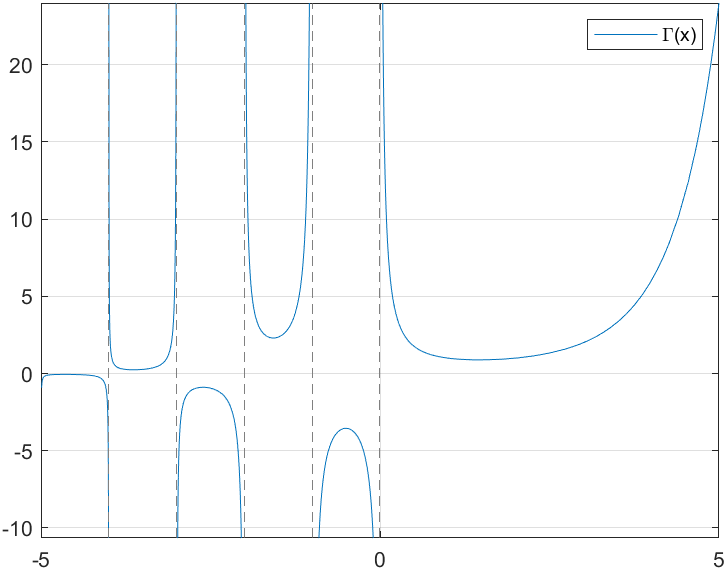
\includegraphics[scale=0.7]{Imagenes/Plot_Gamma.png}
   \caption{Gráfica de la función Gamma $\Gamma (p)$}
   \label{fig:figura_plot_gamma}
\end{figure}
\end{frame}

\subsection{Fórmulas que involucran a \texorpdfstring{$\Gamma (p)$}{G (p)}.}

\begin{frame}
\frametitle{Recuperando más fórmulas}
Como veremos a continuación, el desarrollo de las fórmulas para la función $\Gamma (p)$, se sigue de la definición, por lo que la operación algebraica y de solución de la integral es completamente posible.
\end{frame}
\begin{frame}
\frametitle{Recuperando más fórmulas}
Nos interesa que dispongan de una relación de fórmulas y que puedan ocuparlas en donde sea necesario.
\\
\bigskip
\pause
Aunque las fórmulas son válidas, en el caso que se indique, deberán de demostrar la fórmula que vayan a utilizar.
\end{frame}
\begin{frame}
\frametitle{Evaluando la función}
Evaluemos $\Gamma (1/2)$. Usando la definición:
\pause
\begin{align}
\Gamma \left( \dfrac{1}{2}\right) = \scaleint{6ex}_{\bs 0}^{\infty} \dfrac{1}{\sqrt{t}} \, e^{-t} \dd{t}
\label{eq:ecuacion_05_01}
\end{align}
Toma en cuenta que no importa qué letra usemos para la variable \enquote{muda} de integración en una integral definida.
\end{frame} 
\begin{frame}
\frametitle{Cambiando la variable}
Haciendo el cambio de variable en la ec. (\ref{eq:ecuacion_05_01}):
\pause
\begin{align*}
t = y^{2} \hspace{0.5cm} \Rightarrow \dd{t} = 2 \, y \dd{y}
\end{align*}
\end{frame}
\begin{frame}
\frametitle{Llegamos al resultado}
Entonces tenemos que:
\pause
\begin{align*}
\Gamma \left( \dfrac{1}{2} \right) = \scaleint{6ex}_{\bs 0}^{\infty} \, e^{-y^{2}} \, 2 \, y \dd{y} = 2 \scaleint{6ex}_{\bs 0}^{\infty} \, e^{-y^{2}} \dd{y}
\end{align*}
\end{frame}
\begin{frame}
\frametitle{Usando una variable muda}
Con $x$ como la variable \enquote{muda} de integración:
\pause
\begin{align}
\Gamma \left( \dfrac{1}{2} \right) = 2 \scaleint{6ex}_{\bs 0}^{\infty} \, e^{-x^{2}} \dd{x}
\label{eq:ecuacion_05_02}
\end{align}
\end{frame}
\begin{frame}
\frametitle{Llegando a una integral doble}
Multiplicando las dos integrales de $\Gamma (1/2)$ para luego escribir el resultado como una integral doble:
\pause
\begin{align*}
\left[ \Gamma \left( \dfrac{1}{2} \right) \right]^{2} = 4 \scaleint{6ex}_{\bs 0}^{\infty} \, \scaleint{6ex}_{\bs 0}^{\infty} \, e^{-(x^{2} + y^{2})} \dd{x} \dd{y}
\end{align*}
\end{frame}
\begin{frame}
\frametitle{Resolviendo la integral doble}
Tenemos una doble integral sobre el primer cuadrante de una circunferencia, por lo que es más fácil evaluarla en coordenadas polares:
\pause
\begin{align*}
\left[ \Gamma \left( \dfrac{1}{2} \right) \right]^{2} &= 4 \scaleint{6ex}_{\bs 0}^{\pi/2} \, \scaleint{6ex}_{\bs 0}^{\infty} \, e^{-r^{2}} \, r \dd{r} \dd{\theta} = \\[0.5em]
&= 4 \, \dfrac{\pi}{2} \, \dfrac{e^{-r^{2}}}{-2}\eval_{0}^{\infty} = \\[0.5em]
&= \pi
\end{align*}
\end{frame}
\begin{frame}
\frametitle{Primera expresión}
Entonces obtenemos la primera fórmula:
\pause
\begin{align}\addtolength{\fboxsep}{5pt}\boxed{
\Gamma \left( \dfrac{1}{2} \right) = \sqrt{\pi}}
\label{eq:ecuacion_05_03}
\end{align}
\end{frame}

\subsubsection*{Otras fórmulas}

\begin{frame}
\frametitle{Más expresiones}
A continuación se enlistan algunas de las fórmulas que involucran a la función Gamma, \pause toma en cuenta de que a pesar de que no se demuestra la expresión, en el caso de que la utilices para un ejercicio, deberás de presentar la respectiva demostración.
\end{frame}
\begin{frame}
\frametitle{Expresiones}
{%\fontsize{12}{12}\selectfont
\begin{eqnarray*}
\begin{aligned}
\Gamma (x) &= (x - 1) \, \Gamma(x - 1) \hspace{1cm} x \neq 0, -1, -2, \ldots \\[0.75em] \pause
\Gamma (-x) &= \dfrac{\Gamma (1- x)}{-x} \hspace{1cm} x \neq 0, 1, 2, \ldots \\[0.75em] \pause
\Gamma (x) \, \Gamma (1 - x) &= \dfrac{\pi}{\sin x \, \pi}, \hspace{1.5cm} x \neq 0, \pm 1, \pm 2, \pm 3, \end{aligned}
\end{eqnarray*}
}
\end{frame}
\begin{frame}
\frametitle{Expresiones}
{%\fontsize{12}{12}\selectfont
\begin{eqnarray*}
\begin{aligned}
n! &= \left( \dfrac{n}{e} \right)^{n} \, \sqrt{2 \, \pi \, n} + h \\[0.5em]
&\mbox{con } n = 1, 2, 3, \ldots, \hspace{0.5cm} 0 < \dfrac{h}{n!} < \dfrac{1}{12 \, n} \\[0.5em] \pause
\Gamma \left(n + \dfrac{1}{2} \right) &= \dfrac{1 \cdot 3 \cdot 5 \ldots (2 \, n - 1)\sqrt{\pi}}{2^{n}}, \hspace{0.7cm} n = 1, 2, 3, \ldots
\end{aligned}
\end{eqnarray*}
}
\end{frame}
\begin{frame}
\frametitle{Expresiones}
{%\fontsize{12}{12}\selectfont
\begin{eqnarray*}
\begin{aligned}
\scaleint{6ex}_{\bs 0}^{\infty} t^{a} \, e^{-b \, t^{c}} \dd{t} &= \dfrac{\Gamma \left(\dfrac{a + 1}{c} \right)}{c \, b^{(a+1)/c}}, \\[0.5em]
&\mbox{con } a > -1, \hspace{0.5cm} b > 0, \hspace{0.5cm} c > 0   
\end{aligned}
\end{eqnarray*}
}
\end{frame}

\subsection*{Otras representaciones} \label{seccion:otras_respresentaciones}

\begin{frame}
\frametitle{Diversas representaciones}
Existen al menos tres formas diferentes y convenientes de definir la función Gamma. Se revisarán inicialmente las definiciones así como una serie de consecuencias directas de cada una de ellas.
\end{frame}

\subsubsection{Límite infinito (Euler).}

\begin{frame}
\frametitle{Límite infinito}
La primera definición, llamada de \emph{Euler} es:
\pause
\begin{eqnarray}
\begin{aligned}
\Gamma(z) \equiv \lim_{n \to \infty} &\dfrac{1 \cdot 2 \cdot 3 \cdots n}{z (z + 1) (z + 2) \cdots (z + n)} n^{z}, \\ 
z \neq &0, -1,-2,-3, \ldots
\label{eq:ecuacion_10_01}
\end{aligned}
\end{eqnarray}
\end{frame}
\begin{frame}
\frametitle{Utilidad de la expresión}
Sin pérdida de generalidad, $z$ puede ser real o complejo.
\\
\bigskip
\pause
Esta definición de $\Gamma(z)$ es útil para el desarrollo del producto infinito de Weierstrass de $\Gamma (z)$.
\end{frame}
\begin{frame}
\frametitle{Cambiando la variable}
Reemplazando $z$ con $z + 1$, tenemos:
\pause
\begin{align}
\begin{aligned}[b]
&\Gamma (z + 1) = \\[0.5em]
&= \lim_{n \to \infty} \dfrac{1 \cdot 2 \cdot 3 \cdots n}{(z {+} 1)(z {+} 2)(z {+} 3) \cdots (z {+} n {+} 1)} n^{z {+} 1} = \\[0.5em]
&= \lim_{n \to \infty} \dfrac{n \, z}{z {+} n {+} 1} \: \dfrac{1 \cdot 2 \cdot 3 \cdots n}{z (z {+} 1)(z {+} 2)(z {+} 3) \cdots (z {+} n)} n^{z} \\[0.5em]
&= z \: \Gamma (z)
\label{eq:ecuacion_10_02}
\end{aligned}
\end{align}
\fontsize{12}{12}\selectfont
Esta es la relación funcional básica para la función Gamma.
\end{frame}
\begin{frame}
\frametitle{Característica de la expresión}
Debe notarse que es una ecuación de diferencias. Se ha demostrado que la función Gamma es una de una clase general de funciones que no satisfacen ninguna ecuación diferencial con coeficientes racionales.
\end{frame}
\begin{frame}
\frametitle{De la relación con otra función especial}
Específicamente, la función Gamma es una de las pocas funciones de la física matemática que no satisface tanto la ecuación diferencial hipergeométrica como la ecuación hipergeométrica confluente (que estudiaremos en el \emph{Tema 5 - Funciones Especiales}).
\end{frame}
\begin{frame}
\frametitle{Revisando la expresión}
De la definición:
\pause
\begin{align}
\Gamma (1) = \lim_{n \to \infty} \dfrac{1 \cdot 2 \cdot 3 \cdots n}{1 \cdot 2 \cdot 3 \cdots n \, (n + 1)} \: n = 1
\label{eq:ecuacion_10_03}
\end{align}
\end{frame}
\begin{frame}
\frametitle{Ocupando otra expresión}
Usando de la ecuación (\ref{eq:ecuacion_10_02}), tenemos:
\pause
\begin{align}
\begin{aligned}
\Gamma (2) &= 1 \\
\Gamma (3) &=  2 \: \Gamma(2) =  2 \\
\vdots \\
\Gamma (n) &= 1 \cdot 2 \cdot 3 \cdots (n-1) =  (n-1)!
\label{eq:ecuacion_10_04}
\end{aligned}
\end{align}
\end{frame}

\subsection{Integral definida (Euler)}

\begin{frame}
\frametitle{Segunda definición}
Una segunda definición es la llamada forma de Euler:
\pause
\begin{align}
\Gamma (z) \equiv \scaleint{6ex}_{\bs 0}^{\infty} e^{-t} \: t^{z - 1} \, \dd t, \hspace{1.5cm} \Re(z) > 0
\label{eq:ecuacion_10_05}
\end{align}
La restricción en $z$ es necesaria para prevenir la divergencia de la integral.
\end{frame}
\begin{frame}
\frametitle{Variantes de $\Gamma (z)$}
Cuando la función Gamma aparece en problemas de la física, a menudo tiene una variante:
\pause
\begin{align}
\Gamma (z) &= 2 \: \scaleint{6ex}_{\bs 0}^{\infty} \exp(-t^{2}) \: t^{2 \, z - 1} \dd{t}, \hspace{1cm} \Re(z) > 0  \label{eq:ecuacion_10_06} \\
\Gamma (z) &=  \scaleint{6ex}_{\bs 0}^{1} \left[ \ln\left(\dfrac{1}{t} \right) \right]^{z - 1} \dd{t}, \hspace{1cm} \Re (z) > 0 \label{eq:ecuacion_10_07}
\end{align}
\end{frame}
\begin{frame}
\frametitle{Recuperando otra función}
Cuando $z = 1/2$, la ecuación (\ref{eq:ecuacion_10_06}) es la función de error gaussiana, que nos devuelve el siguiente resultado interesante:
\pause
\begin{align}
\Gamma (1/2) = \sqrt{\pi}
\label{eq:ecuacion_10_08}
\end{align}
\end{frame}
\begin{frame}
\frametitle{Demostrando la relación}
Para mostrar la equivalencia de esas dos definiciones, las ecuaciones (\ref{eq:ecuacion_10_01}) y (\ref{eq:ecuacion_10_05}) consideremos la función de dos variables:
\pause
\begin{align}
F(z, n) = \scaleint{6ex}_{\bs 0}^{n} \left( 1 - \dfrac{t}{n} \right)^{n} \: t^{z - 1} \dd{t}, \hspace{1.5cm} \Re(z) > 0
\label{eq:ecuacion_10_09}
\end{align}
con $n$ entero positivo.
\end{frame}
\begin{frame}
\frametitle{Revisando la expresión}
Ya que:
\pause
\begin{align}
\lim_{n \to \infty} \left( 1 - \dfrac{t}{n} \right)^{n} \equiv e^{-t}
\label{eq:ecuacion_10_10}
\end{align}
\end{frame}
\begin{frame}
\frametitle{Ocupando al definición}
De la definición de función exponencial:
\pause
\begin{equation}
\begin{aligned}[b]
&\lim_{n \to \infty} F(z, n) = F (z, \infty) = \\[0.5em]
&= \scaleint{6ex}_{\bs 0}^{\infty} \exp(-t) \: t^{z - 1} \dd{t} \equiv \Gamma (z)
\end{aligned}
\label{eq:ecuacion_10_11}
\end{equation}
por la ecuación (\ref{eq:ecuacion_10_05}).
\end{frame}
\begin{frame}
\frametitle{Regresando a la expresión}
Regresando a $F (z, n)$, evaluamos sucesivamente la integral por partes, hacemos de manera conveniente $u = t/n$. Entonces:
\pause
\begin{align}
F (z, n) = n^{2} \: \scaleint{6ex}_{\bs 0}^{1} (1-u)^{n} \: u^{z-1} \dd{u}
\label{eq:ecuacion_10_12}
\end{align}
\end{frame}
\begin{frame}
\frametitle{Integrando la expresión}
Integrando por partes:
\pause
\begin{eqnarray}
\begin{aligned}[b]
&\dfrac{F (z, n)}{n^{2}} =  (1-u)^{n} \: \dfrac{u^{z}}{z} \eval_{0}^{1} + \\
&+ \dfrac{n}{z} \: \scaleint{6ex}_{\bs 0}^{1} (1-u)^{n-1} \: u^{z} \dd{u}
\end{aligned}
\label{eq:ecuacion_10_13}
\end{eqnarray}
\end{frame}
\begin{frame}
\frametitle{Repitiendo el cálculo}
Repitiendo esto cada vez con el integrando se anula en ambos extremos, por lo que:
\pause
\begin{align}
\begin{aligned}[b]
F (z, n) &= n^{z} \: \dfrac{n(n-1) \cdots 1}{z \, (z+1) \cdots (z+n-1)} \scaleint{6ex}_{\bs 0}^{1} u^{z+n-1} \dd{u} \\[0.5em]
&= \dfrac{1 \cdot 2 \cdot 3 \cdots n}{z \, (z+1)(z+2) \cdots (z+n)} \: n^{z}
\label{eq:ecuacion_10_14}
\end{aligned}
\end{align}
\end{frame}
\begin{frame}
\frametitle{Identificando el resultado}
Que es idéntico con la expresión del lado derecho de la ecuación (\ref{eq:ecuacion_10_01}). De aquí que:
\pause
\begin{equation}
\lim_{n \to \infty} F(z, n) = F(z, \infty) \equiv \Gamma (z)
\label{eq:ecuacion_10_15}
\end{equation}
\end{frame}

\subsection{Producto infinito (Weierstrass)}

\begin{frame}
\frametitle{Tercera definición}
La tercera forma conocida como forma de Weierstrass es:
\pause
\begin{align}
\dfrac{1}{\Gamma (z)} \equiv z \:  e^{\gamma \, z} \: \prod_{n=1}^{\infty} \left( 1 + \dfrac{z}{n} \right) \: e^{-z/n}
\label{eq:ecuacion_10_16}
\end{align}
donde $\gamma$ es la constante de \emph{Euler-Mascheroni}:
\begin{align}
\gamma = 0.5772156619
\label{eq:ecuacion_10_17}
\end{align}
\end{frame}
\begin{frame}
\frametitle{Resultado de utilidad}
De esta definición de producto infinito de $\Gamma (z)$, se obtiene una identidad importante:
\pause
\begin{align}
\Gamma (z) \: \Gamma (1 - z) = \dfrac{\pi}{\sin z \, \pi}
\label{eq:ecuacion_10_23}
\end{align}
\end{frame}
\begin{frame}
\frametitle{Otro resultado}
Así también la \textbf{fórmula de duplicación de Legendre}:
\pause
\begin{align}
\Gamma (1 + z) \: \Gamma (z + \frac{1}{2}) = 2^{-2 \, z} \: \sqrt{\pi} \: \Gamma (2 \, z + 1)
\label{eq:ecuacion_10_24b}
\end{align}
\end{frame}
\begin{frame}
\frametitle{Polos en la función}
La definición de Weierstrass muestra directamente que $\Gamma (z)$ tiene polos simples en $z = 0, -1, -2, -3, \ldots$ y que $[\Gamma (z)]^{-1}$ no tiene polos en el plano complejo finito, lo que significa que $\Gamma (z)$ no tiene ceros.
\end{frame}

\subsection{Funciones Digamma y Poligamma}

\subsection*{La función Digamma}

\begin{frame}
\frametitle{Función Digamma}
No es conveniente manejar las derivadas de las funciones Gamma o factorial de manera directa, como se definieron en la sección (\ref{seccion:otras_respresentaciones}).
\end{frame}
\begin{frame}
\frametitle{Ajuste en la expresión}
Para evitar ese manejo, lo que se hace es tomar el logaritmo natural de la función factorial (\ref{eq:ecuacion_10_01}), cambiando el producto a una suma y luego se realiza la diferenciación, es decir:
\pause
\begin{align}
z! = \lim_{n \to \infty} \dfrac{n!}{(z + 1)(z + 2) \ldots (z + n)} \, n^{z}
\label{eq:ecuacion_10_36}
\end{align}
\end{frame}
\begin{frame}
\frametitle{Tomando el logaritmo natural}
Que al tomar el logaritmo natural, resulta:
\pause
\begin{align}
\begin{aligned}
\ln (z!) &= \lim_{n \to \infty} \big[ \ln (n!) + z \, \ln n - \ln (z + 1) + \\[0.5em]
&- \ln (z + 2) - \ldots - \ln (z + n) \big]
\end{aligned}
\label{eq:ecuacion_10_37}
\end{align}
en donde el logaritmo del límite es igual al límite del logaritmo
\end{frame}
\begin{frame}
\frametitle{Diferenciando la expresión}
Al diferenciar con respecto a $z$, se obtiene:
\pause
\begin{align}
\begin{aligned}[b]
&\dv{\ln (z!)}{z} \equiv \psi(z + 1) = \\[0.5em]
&=\lim_{n \to \infty} \bigg[ \ln n {+} z - \dfrac{1}{(z {+} 1)} - \dfrac{1}{(z {+} 2)} \ldots - \dfrac{1}{(z {+} n)} \bigg]
\end{aligned}
\label{eq:ecuacion_10_38}
\end{align}
\end{frame}
\begin{frame}
\frametitle{La función digamma}
La cual define a la \emph{función digamma}. De la expresión para la constante de Euler-Mascheroni, la ec. (\ref{eq:ecuacion_10_38}) se puede reescribir como:
\pause
\begin{align}
\begin{aligned}[b]
\psi (z + 1) &= - \gamma - \sum_{n=1}^{\infty} \left( \dfrac{1}{z + n} - \dfrac{1}{n} \right) = \\[0.5em]
&= -\gamma + \sum_{n=1}^{\infty} \dfrac{z}{n (n + z)}
\end{aligned}
\label{eq:ecuacion_10_39}
\end{align}
\end{frame}

\subsection*{Función Poligamma.}

\begin{frame}
\frametitle{Diferenciando nuevamente}
La función Digamma se puede diferenciar de manera iterativa, dando origen a la función Poligamma:
\pause
\begin{align}
\begin{aligned}
&\ntilde{\psi}{m} (z + 1) \equiv \dv[m+1]{z} \ln(z!) = \\[0.5em]
&= (-1)^{m+1} \, m! \,\sum_{n=1}^{\infty} \dfrac{1}{(z + n)^{m+1}}, \hspace{1cm} m = 1, 2, 3, \ldots
\end{aligned}
\label{eq:ecuacion_10_41}
\end{align}
\end{frame}
\section{Función Beta}
\frame[allowframebreaks]{\tableofcontents[currentsection, hideothersubsections]}
\subsection{Definición}
\begin{frame}[fragile]
\frametitle{Definición de la función Beta}
La función Beta se define por la siguiente integral:
\begin{align} \addtolength{\fboxsep}{5pt}\boxed{
\begin{gathered}
B(p, q) = \scaleint{6ex}_{\bs 0}^{1} x^{p-1} \, (1- x )^{q-1} \dd{x}, \\
\mbox{con }  p > 0, q > 0
\end{gathered}
}
\label{eq:ecuacion_06_01}
\end{align}
\pause
Existen una serie de fórmulas para la función Beta que es conveniente conocer, todas ellas derivadas de la definición.
\end{frame}
\begin{frame}
\frametitle{Fórmulas para $B(p, q)$}
Si cambiamos el rango de integración de la ec. (\ref{eq:ecuacion_06_01}), haciendo $x = y/a$, entonces $x = 1$ corresponde a $y = a$, por lo que tenemos:
\begin{align} \addtolength{\fboxsep}{5pt}\boxed{
\begin{aligned}
B (p, q) &= \scaleint{6ex}_{\bs 0}^{a} \left( \dfrac{y}{a}\right)^{p-1} \, \left( 1 - \dfrac{y}{a}\right)^{q-1} \dfrac{\dd{y}}{a} \\[0.5em]
&= \dfrac{1}{a^{p+q-1}} \scaleint{6ex}_{\bs 0}^{a} y^{p-1} \, (a - y)^{q-1} \dd{y}
\end{aligned}
\label{eq:ecuacion_06_03}
}
\end{align}
\end{frame}
\subsection{Fórmula trigonométrica de \texorpdfstring{$B(p,q)$}{B(p, q)}}
\begin{frame}
\frametitle{Fórmula trigonométrica de $B(p,q)$}
Para obtener la forma trigonométrica de la función Beta, hacemos el cambio de variable $x = \sin^{2} \theta$, así
\begin{align*}
\dd{x} &= 2 \, \sin \theta \, \cos \theta \dd{\theta} \\[1em]
(1 - x) &= 1 - \sin^{2} \theta = \cos^{2} \theta \\[1em]
x &= 1 \hspace{0.3cm} \Rightarrow \hspace{0.3cm} \theta = \pi/2
\end{align*}
\end{frame}
\begin{frame}
\frametitle{Fórmula trigonométrica de $B(p, q)$}
Haciendo las sustituciones en la ec. (\ref{eq:ecuacion_06_01}):
{\fontsize{12}{12}\selectfont
\begin{align}
B(p, q) = \scaleint{6ex}_{\bs 0}^{\pi/2} \left( \sin^{2} \theta \right)^{p-1} \, \left( \cos^{2} \theta \right)^{q-1} \, 2 \, \sin \theta \, \cos \theta \dd{\theta}
\end{align}}
\pause
Simplificando la expresión llegamos a:
{\fontsize{12}{12}\selectfont
\begin{align}
\addtolength{\fboxsep}{5pt}\boxed{B(p, q) = 2 \, \scaleint{6ex}_{\bs 0}^{\pi/2} \left( \sin^{2} \theta \right)^{2p-1} \, \left( \cos^{2} \theta \right)^{2q-1} \dd{\theta}}
\label{eq:ecuacion_06_04}
\end{align}}
\end{frame}
\begin{frame}
\frametitle{Otra fórmula para $B(p, q)$}
Con el cambio de variable en la ec. (\ref{eq:ecuacion_06_01})
\begin{align*}
x = \dfrac{y}{(1 + y)}
\end{align*}
\pause
Se puede demostrar que
\begin{align}
\addtolength{\fboxsep}{5pt}\boxed{B(p, q) = \scaleint{6ex}_{\bs 0}^{\infty} \dfrac{y^{p-1}}{(1 + y)^{p+q}} \dd{y}}
\label{eq:ecuacion_06_05}
\end{align}   
\end{frame}
\begin{frame}
\frametitle{Otras fórmulas}
Como en el caso de la función $\Gamma (x)$, las fórmulas que se presentan para $B(p, q)$ se demuestran a partir de la definición y de un manejo algebraico, por lo que en caso de que utilices alguna en la solución de un ejercicio, tendrás que demostrar la fórmula.
\end{frame}
\begin{frame}
\frametitle{Otras fórmulas}
\begin{align*}
B (x, y) &= B (y, x) \\[1em]
B (x, 2-x) &= \dfrac{\pi}{\sin x \, \pi}, \hspace{1.5cm} 0 < x < 1   
\end{align*}
\end{frame}
\subsection{La función Beta en términos de Gamma}
\begin{frame}
\frametitle{La función $B(p, q)$ en términos de $\Gamma (p)$}
La función Beta se expresa en términos de la función Gamma de la siguiente manera:
\begin{align}
\addtolength{\fboxsep}{5pt}\boxed{B(p, q) = \dfrac{\Gamma(p) \, \Gamma(q)}{\Gamma (p + q)}}
\label{eq:ecuacion_07_01}
\end{align}
Esta fórmula nos ayuda a evaluar una función $B (p, q)$ en términos de funciones $\Gamma$. \textbf{Nota: } también es fácil demostrar la expresión, para que en el caso de que la utilices, realices el ejercicio.
\end{frame}
\section{Ejemplos}
\frame[allowframebreaks]{\tableofcontents[currentsection, hideothersubsections]}
%Referencia: Farrell - Solved Problems in Analysis as Applied to Gamma Function II-39
\subsection{Longitud de una lemniscata}
\begin{frame}
\frametitle{Longitud de una leminiscata}
Usando la función Gamma, calcula la longitud de la lemniscata
\begin{align*}
\rho^{2} = a^{2} \, \cos 2 \theta
\end{align*}
\end{frame}
\begin{frame}
\frametitle{Longitud de una leminiscata}
\begin{wrapfigure}{r}{0.55\textwidth}
    \centering
    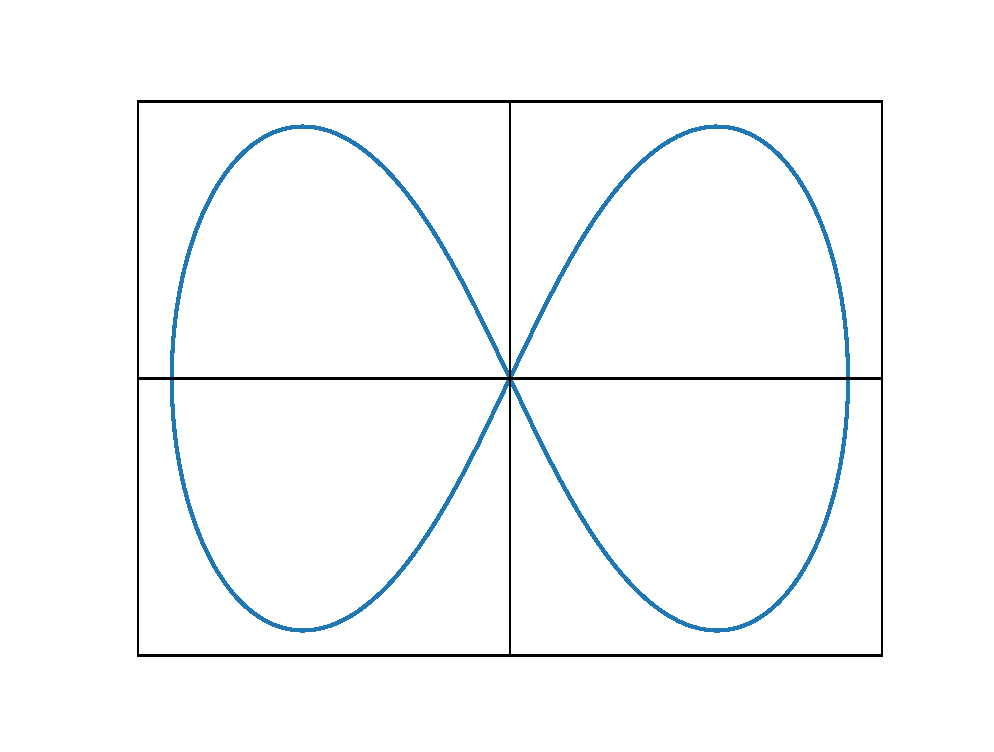
\includegraphics[scale=0.35]{Imagenes/plot_leminscata_01.eps}
    \caption{Gráfica de la lemniscata.}
    \label{fig:figura_lemniscata}
\end{wrapfigure}
La curva se parece a un ocho invertido, teniendo al eje x como eje de simetría, pasa en dos ocasiones por el origen, como se puede ver en la figura (\ref{fig:figura_lemniscata})
\end{frame}
\begin{frame}
\frametitle{Tomando la simetría del problema}
Para esta curva, por simetría se tiene la misma longitud en cada uno de los cuatro cuadrantes, por lo que podemos calcular la longitud en el primer cuadrante y luego multiplicarla por cuatro.
\end{frame}
\begin{frame}
\frametitle{Tomando la simetría del problema}
Los puntos donde la curva cruza el eje $x$ en el origen son aquellos para los cuales el argumento del coseno es un múltiplo entero, impar de $\pi / 2$. 
\\
\bigskip
Para el tramo en el primer cuadrante, tomamos $0 \leq \theta \leq \pi/4$.
\end{frame}
\begin{frame}
\frametitle{Resolviendo el problema}
La longitud de la curva en coordenadas polares es
\begin{align*}
s = \scaleint{6ex}_{\bs \alpha}^{\beta} \left[ \rho^{2} + \left( \dv{\rho}{\theta} \right)^{2} \right]^{1/2} \dd{\theta}
\end{align*}
\pause
Como $\rho^{2} = a^{2} \, \cos 2 \theta$, tenemos que:
\begin{align*}
\left( \dv{\rho}{\theta} \right)^{2} = \dfrac{a^{4} \, \sin^{2} 2 \theta}{a^{2} \, \cos 2 \theta}
\end{align*}
\end{frame}
\begin{frame}
\frametitle{Resolviendo el problema}
Entonces:
\begin{align*}
\dfrac{1}{4} \, s &= \scaleint{6ex}_{\bs {0}}^{\pi/4} \left( a^{2} \, \cos 2 \theta + \dfrac{a^{4} \, \sin^{2} 2 \theta}{\cos 2 \theta} \right)^{1/2} \dd{\theta} = \\[1em]
&= \scaleint{6ex}_{\bs {0}}^{\pi/4} a \, \cos^{-1/2} 2 \theta \dd{\theta}
\end{align*}
\end{frame}
\begin{frame}
\frametitle{Resolviendo al integral}
Haciendo un cambio de variable, es posible llevar esta integral a uno forma de la función Beta con integral.
\\
\bigskip
Sea $2 \theta = t$. Por lo que el intervalo de integración ahora va de $0$ a $\pi/2$.
\end{frame}
\begin{frame}
\frametitle{Resolviendo la integral}
Por tanto:
\begin{align*}
\scaleint{6ex}_{\bs 0}^{\pi/4} a \, \cos^{-1/2} \, 2 \, \theta \dd{\theta} = \dfrac{a}{2} \scaleint{6ex}_{\bs {0}}^{\pi/2} \cos^{-1/2} \, t \, \sin^{0} t \dd{t}
\end{align*}
\end{frame}
\begin{frame}
\frametitle{Resolviendo la integral}
De uno de los resultados para la función Beta:
\begin{align*}
B(x, y) = \scaleint{6ex}_{\bs {0}}^{\pi/2} 2 \, \sin^{2x-1} \theta \, \cos^{2y-1} \theta \dd{\theta}
\end{align*}
\pause
por tanto
\begin{align*}
\dfrac{1}{4} \, s &= \scaleint{6ex}_{\bs {0}}^{\pi/4} a \, \cos^{-1/2} 2 \theta \dd{\theta} =  \\[0.5em]
&= \dfrac{a}{2} \scaleint{6ex}_{\bs {0}}^{\pi/2} \cos^{-1/2} t \, \sin^{0} t \dd{t}
\end{align*}
\end{frame}
\begin{frame}
\frametitle{Resolviendo la integral}
Encontramos entonces que
\begin{align*}
\dfrac{1}{4} \, s &= \dfrac{a}{2} \, \dfrac{1}{2} \, B \, \left(\dfrac{1}{4}, \dfrac{1}{2} \right) = \\[1em]
&= \dfrac{a}{4} B\left(\dfrac{1}{4}, \dfrac{1}{2} \right)
\end{align*}
\pause
\fontsize{12}{12}\selectfont
La longitud completa de la lemniscata se obtiene al multiplicar el resultado anterior por cuatro, además ocupamos la fórmula que relaciona la función Beta con la función Gamma.
\end{frame}
\begin{frame}
\frametitle{Solución al problema}
Así tenemos el resultado:
\begin{eqnarray*}
s &=& a \, B\left(\dfrac{1}{4}, \dfrac{1}{2} \right) = \dfrac{a \, \Gamma \left( \dfrac{1}{4} \right) \, \Gamma \left( \dfrac{1}{2} \right) }{\Gamma \left( \dfrac{3}{4} \right)} = \\ \pause
&=& \dfrac{4 \, a \, \Gamma \left( \dfrac{5}{4} \right) \sqrt{\pi}}{\dfrac{4}{3} \, \Gamma \left( \dfrac{7}{4} \right)} \pause \cong 5.2 \, a
\end{eqnarray*}
\end{frame}

\subsection{Período de oscilación de un péndulo.}

\begin{frame}
\frametitle{Problema de mecánica}
Se nos pide calcular el período de oscilación de un péndulo simple que oscila en un arco de $\ang{180}$, como se aprecia en la figura (\ref{fig:figura_pendulo_simple}):
\end{frame}
\begin{frame}
\frametitle{Problema de mecánica}
\begin{figure}[!ht]
    \centering
    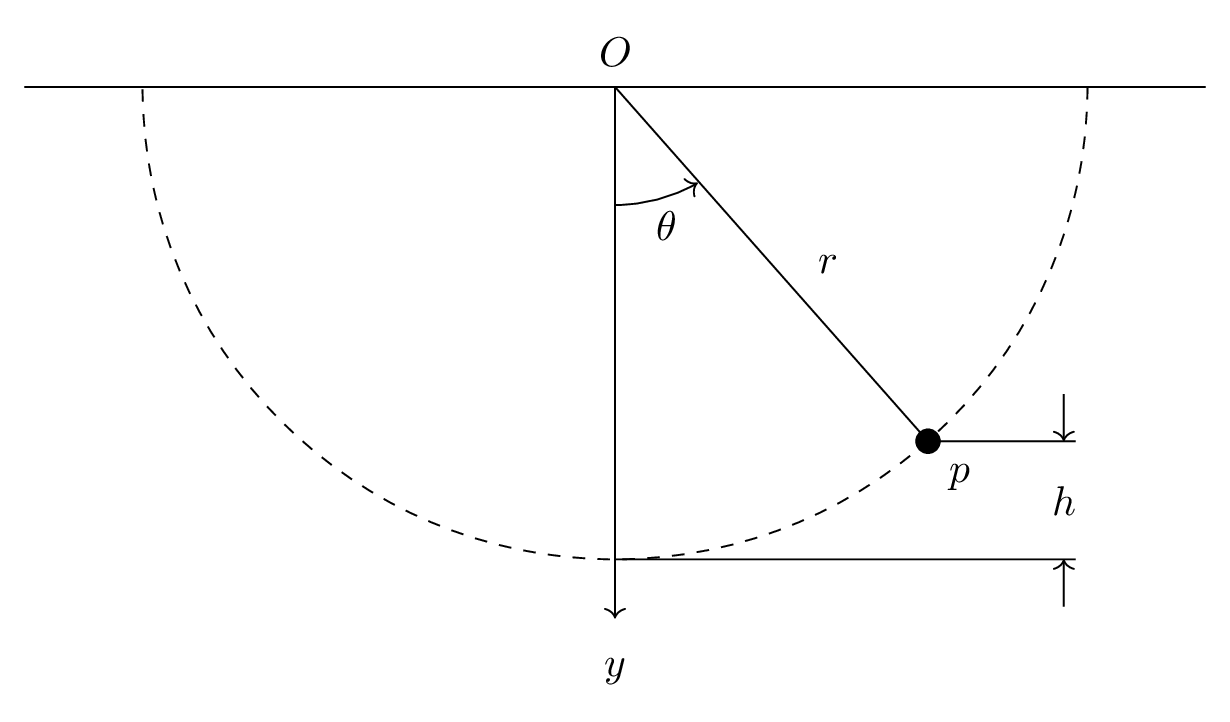
\includegraphics{Imagenes/pendulo_simple.pdf}
    \caption{Esquema del péndulo simple que oscila en un arco.}
    \label{fig:figura_pendulo_simple}
\end{figure}
\end{frame}
\begin{frame}
\frametitle{Organizando el problema}
Usando el eje coordenado, vemos que el ángulo polar $\theta$ varía de $-\pi/2$ a $\pi/2$, mientras que la coordenada radial $r = Op$ permanece constante.
\end{frame}
\begin{frame}
\frametitle{Organizando el problema}
Sea $g$ la aceleración debida a la gravedad y $W$ el peso del péndulo $p$.
\\
\bigskip
\pause
La energía potencial de $p$ en $\theta = 0$ es cero. Por lo que el valor de la energía potencial en cualquier instante, es el producto de $W$ por la altura $h$:
\pause
\begin{align*}
P = W (r - r \, \cos \theta)
\end{align*}
\end{frame}
\begin{frame}
\frametitle{Organizando el problema}
Mientras que la energía cinética viene dada por:
\pause
\begin{align*}
K = \dfrac{m \, v^{2}}{2} = \dfrac{1}{2} \, \dfrac{W}{g} \left( r \, \dv{\theta}{t} \right)^{2}
\end{align*}
Como el péndulo está oscilando, la energía total es constante: $P + K = C$.
\end{frame}
\begin{frame}
\frametitle{Organizando el problema}
Lo que nos permite expresar una ecuación diferencial del movimiento:
\pause
\begin{align*}
W \, r (1 - \cos \theta) + \dfrac{1}{2} \dfrac{W}{g} \left( r \dv{\theta}{t} \right)^{2} = C
\end{align*}
\end{frame}
\begin{frame}
\frametitle{Condiciones para la ec. diferencial}
Para calcular $C$ tomamos el tiempo $t = 0$ cuando $\theta = \pi/2$, vemos que el péndulo está en reposo, por lo que $\dv*{\theta}{t} = 0$, cuando $t = 0$ y $\theta = \pi/2$.
\end{frame}
\begin{frame}
\frametitle{Ecuación de movimiento}
De esta manera $C = W \, r$ y la ecuación de movimiento resulta:
\pause
\begin{align*}
\dfrac{r}{2 \, g} \left( \dv{\theta}{t} \right)^{2} - \cos \theta = 0
\end{align*}
\end{frame}
\begin{frame}
\frametitle{Consideración}
Como $p$ está oscilando de un lado a otro, $\dv*{\theta}{t}$ es en ocasiones positiva y en otras negativa; podemos estimar el período $T$, calculando el tiempo que tarda de ir de $\theta = 0$ a $\theta = \pi/2$, para luego multiplicar el resultado por $4$.
\\
\bigskip
\pause
De esta manera podemos usar la raíz positiva para resolver la ecuación de $\dv*{\theta}{t}$.
\end{frame}
\begin{frame}
\frametitle{Resolviendo la ecuación diferencial}
Entonces tenemos:
\pause
\begin{eqnarray*}
\begin{aligned}
\sqrt{\dfrac{r}{2 \, g}} \, \dv{\theta}{t} &= \cos^{1/2} \theta \dd{t} = \\[1em] \pause
\dd{t} &= \sqrt{\dfrac{r}{2 \, g}} \, \dv{\theta}{t} \cos^{-1/2} \theta \dd{\theta} = \\[1em] \pause
T &= 4 \, \sqrt{\dfrac{r}{2 \, g}} \, \scaleint{6ex}_{\bs {0}}^{\pi/2} \cos^{-1/2} \theta \dd{\theta} =
\end{aligned}
\end{eqnarray*}
\end{frame}
\begin{frame}
\frametitle{Resolviendo la ecuación diferencial}
Se sigue que:
\begin{eqnarray*}
\begin{aligned}
&= 2 \, \sqrt{\dfrac{r}{2 \, g}} \, \scaleint{6ex}_{\bs {0}}^{\pi/2} 2 \, \sin^{0} \theta \, \cos^{-1/2} \theta \dd{\theta} = \\[0.8em] \pause
&= \sqrt{\dfrac{2 \, r}{g}} \, B \left( \dfrac{1}{2}, \dfrac{1}{4} \right) = \\[0.8em] \pause
&= \sqrt{\dfrac{2 \, r}{g}} \, \dfrac{\Gamma \left(\dfrac{1}{2} \right) \, \Gamma \left(\dfrac{1}{4} \right)}{\Gamma \left(\dfrac{3}{4} \right)} = 
\end{aligned}
\end{eqnarray*}
\end{frame}
\begin{frame}
\frametitle{Resolviendo la ecuación diferencial}
\begin{eqnarray*}
\begin{aligned}
T &= \sqrt{\dfrac{2 \, r}{g}} \, \dfrac{\Gamma \left(\dfrac{1}{2} \right) \, 4 \, \Gamma \left(\dfrac{5}{4} \right)}{\dfrac{4}{3} \, \Gamma \left(\dfrac{7}{4} \right)} = \\[0.5em] \pause
&= \sqrt{\dfrac{2 \, r}{g}} \, \left[ \dfrac{3 \sqrt{\pi } \Gamma \left(\dfrac{5}{4}\right)}{\Gamma \left(\dfrac{7}{4}\right)} \right] = \\[0.5em] \pause
&= 5.24412 \, \sqrt{\dfrac{2 \, r}{g}}
\end{aligned}
\end{eqnarray*}
\end{frame}

\subsection{Segundo ejercicio de la mecánica}

\begin{frame}
\frametitle{Enunciado del problema}
Una partícula de masa $m$ en el eje $x$ positivo es atraía hacia el origen por una fuerza variable tal que el producto de la magnitud de la fuerza por la distancia desde el origen es una constante $k$. La partícula parte del reposo en $x = L$.
\\
\bigskip
\pause
\textocolor{blue}{Determina el tiempo necesario para que la partícula llegue el origen.}
\end{frame}
\begin{frame}
\frametitle{El problema}
Con un esquema tenemos que nuestro problema es:
\begin{figure}
    \centering
    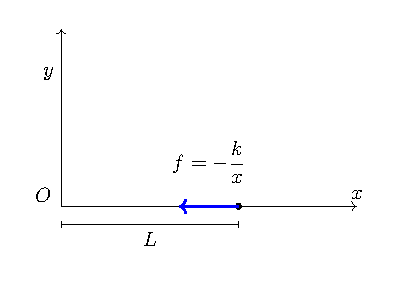
\includegraphics[scale=1]{Imagenes/Ejercicio_Gamma_Particula.eps}
    \caption{La partícula desplazándose hacia el origen.}
\end{figure}
\end{frame}
\begin{frame}
\frametitle{Usando la física para la solución}
Partimos de la segunda ley de Newton $F = m \, a$, vemos que la única componente que permanece es en la dirección del eje $x$.
\\
\bigskip
\pause
Entonces tenemos que:
\begin{align*}
- \dfrac{k}{x} = m \, \dv[2]{x}{t}
\end{align*}
\end{frame}
\begin{frame}
\frametitle{Manejando la expresión}
Acomodemos los términos y multipliquemos ambos lados por $\dv*{x}{t}$:
\pause
\begin{align*}
m \left( \dv[2]{x}{t} \right) \left( \dv{x}{t} \right) = - \dfrac{k}{t} \,  \left( \dv{x}{t} \right)
\end{align*}
\pause
Entonces podemos integrar ambos lados de la igualdad:
\end{frame}
\begin{frame}
\frametitle{Consideración de una derivada}
Tomemos en cuenta que la derivada:
\pause
\begin{align*}
\left[ \left( \dv{x}{t} \right)^{2} \right]^{\prime} = 2 \, \left( \dv{x}{t} \right) \left( \dv[2]{x}{t} \right)
\end{align*}
\pause
Entonces nos queda por resolver:
\pause
\begin{align*}
\dfrac{1}{2} \, m \, \left( \dv{x}{t} \right)^{2} = - k \scaleint{6ex}_{L}^{x} \dfrac{\left( \dv{x}{t} \right)}{x} \dd{t}
\end{align*}
\end{frame}
\begin{frame}
\frametitle{Ocupando la condición inicial}
Consideramos ahora la condición inicial:
\pause
\begin{align*}
\dv{x}{t} = 0 \hspace{1cm} \mbox{cuando } x = L
\end{align*}
\pause
Resolvemos la ecuación para la velocidad $\dv*{x}{t}$, tomamos el valor negativo de la raíz cuadrada ya que el movimiento se presenta en la dirección negativa del eje $x$.
\end{frame}
\begin{frame}
\frametitle{Integrando la expresión}
Separamos las variables e integramos:
\pause
\begin{align*}
t = - \sqrt{\dfrac{m}{2 \, k}} \scaleint{6ex}_{\bs L}^{0} \left( \ln \dfrac{L}{x} \right)^{-1/2} \dd{x}
\end{align*}
\pause
Al parecer se complica con respecto a la integración!
\end{frame}
\begin{frame}
\frametitle{Uso de una identidad}
Vamos a ocupar una identidad (que pronto demostraremos):
\begin{align}
\scaleint{6ex}_{\bs 0}^{\infty} t^{a} \, \exp(-b \, t^{c}) \dd{t} = \dfrac{\Gamma \left( \dfrac{a + 1}{c} \right)}{c \, b^{(a+1)/c}}
\label{eq:identidad_Gamma}
\end{align}
donde $b$ y $c$ son constantes positivas, mientras que $a$ es una constante tal que $a > - 1$.
\end{frame}
\begin{frame}
\frametitle{Otra resultado}
Consideremos la siguiente integral:
\pause
\begin{align*}
\scaleint{6ex}_{\bs 0}^{1} x^{m} \, \left( \ln \dfrac{1}{x} \right)^{n} \dd{x} \hspace{1cm} m > -1, n > -1
\end{align*}
\pause
Hacemos el siguiente cambio de variable:
\begin{align*}
\ln \left(\dfrac{1}{x} \right) = t
\end{align*}
\end{frame}
\begin{frame}
\frametitle{Otro resultado}
Con el cambio de variable tenemos que:
\begin{eqnarray*}
\begin{aligned}
\dfrac{1}{x} &= e^{t} \\[0.5em] \pause
x &= e^{-t} \\[0.5em] \pause
x^{m} &= e^{-m t} \\[0.5em] \pause
\dd{x} &= - e^{-t} \dd{t}
\end{aligned}
\end{eqnarray*}
\end{frame}
\begin{frame}
\frametitle{Otro resultado}
Entonces al reexpresar la integral con el cambio de variable y considerando que al invertir los límites de integración, se cancela el signo negativo, tendremos que:
\pause
\begin{align*}
\scaleint{6ex}_{\bs 0}^{1} x^{m} \, \left( \ln \dfrac{1}{x} \right)^{n} \dd{x} = \scaleint{6ex}_{\bs 0}^{\infty} t^{n} \, \exp(-(m+1) \, t) \dd{t}
\end{align*}
\end{frame}
\begin{frame}
\frametitle{Otro resultado}
Utilizando la propiedad (\ref{eq:identidad_Gamma}), con $a = n$, $b = m + 1$ y $c = 1$, el valor de la integral es:
\pause 
\begin{align}
\scaleint{6ex}_{\bs 0}^{1} x^{m} \, \left( \ln \dfrac{1}{x} \right)^{n} \dd{x} = \dfrac{\Gamma (n + 1)}{(m + 1)^{n+1}}
\label{eq:ecuacion_propiedad_Gamma}
\end{align}
\end{frame}
\begin{frame}
\frametitle{Regresando al problema}
Una vez revisados los dos resultados anteriores, para el problema de la partícula moviéndose al origen, entonces hacemos el cambio de variable $x = L \, u$ para obtener:
\pause 
\begin{align*}
t = L \, \sqrt{\dfrac{m}{2 \, k}} \, \scaleint{6ex}_{\bs 0}^{1} u^{0} \, \left( \ln \dfrac{1}{c} \right)^{-1/2} \dd{u}
\end{align*}
\pause
Del resultado obtenido en la ec. (\ref{eq:ecuacion_propiedad_Gamma})
\end{frame}
\begin{frame}
\frametitle{Solución al ejercicio}
Entonces tenemos que: $m = 0$ y $n = -1/2$, por lo que:
\pause
\begin{eqnarray*}
\begin{aligned}
t &= L \, \sqrt{\dfrac{m}{2 \, k}} \, \Gamma(-1/2 + 1) = \pause L \, \sqrt{\dfrac{m}{2 \, k}} \, \Gamma(1/2) = \\[0.5em] \pause
&= L \, \sqrt{\dfrac{m}{2 \, k}} \, \sqrt{\pi} = \\[0.5em] \pause
t &= L \, \sqrt{\dfrac{m \, \pi}{2 \, k}} \qed
\end{aligned}
\end{eqnarray*}
\end{frame}

\section{Identidades Función Gamma}
\frame[allowframebreaks]{\tableofcontents[currentsection, hideothersubsections]}

\subsection{Introducción}
\begin{frame}
\frametitle{Las identidades para la función Gamma}
Ya conocemos la función Gamma a partir de al menos tres definiciones que se revisaron en el material de trabajo.
\\
\bigskip
\pause
Así mismo, conocemos una serie de identidades tanto para la función Gamma y Beta.
\end{frame}
\begin{frame}
\frametitle{Las identidades para la función Gamma}
Aunque las identidades que se han presentado en una lista, son útiles para simplificar el trabajo en la solución de un problema, es conveniente realizar la demostración de las identidades, siendo un ejercicio muy atractivo para reforzar las definiciones de las funciones.
\end{frame}
\begin{frame}
\frametitle{Las identidades para la función Gamma}
En esta sesión demostraremos algunas propiedades de esa lista, como buen ejercicio moral, podrías demostrar las identidades faltantes.
\end{frame}

\subsection{Identidad 1}

\begin{frame}
\frametitle{Propiedad de la función $\Gamma(x)$}
\textbf{Demuestra} la siguiente identidad:
\begin{align*}
\Gamma (x + 1) = x \, \Gamma (x)
\end{align*}
\end{frame}
\begin{frame}
\frametitle{Solución}
Antes de demostrar la identidad directamente de la integral Gamma para todo valor de $x$ positivo, veamos que esta identidad se usa para definir la función Gamma primero para $-1 < x < 0$ escribiéndola en la forma:
\begin{align*}
\Gamma(x) = \dfrac{\Gamma (x + 1)}{x}
\end{align*}
\end{frame}
\begin{frame}
\frametitle{Solución}
Tendremos entonces que la expresión es válida para el intervalo $-2 < x < -1$, y así sucesivamente para todos los valores no enteros negativos de $x$.
\\
\bigskip
\pause
Por lo que nos queda demostrar que se cumple
\begin{align*}
\Gamma (x + 1) =  x \, \Gamma (x)
\end{align*}
para todo $x$ positivo.
\end{frame}
\begin{frame}
\frametitle{Demostración}
Haciendo que $x$ sea cualquier número positivo, escribimos la integral Gamma para el argumento $x + 1$:
\begin{eqnarray*}
\Gamma (x + 1) &= \displaystyle \scaleint{6ex}_{\bs 0}^{\infty} t^{(x+1)-1} \, e^{-t} \dd{t} = \\[1em] \pause
&= \displaystyle \scaleint{6ex}_{\bs 0}^{\infty} t^{x} \, e^{-t} \dd{t}
\end{eqnarray*}
\end{frame}
\begin{frame}
\frametitle{Demostración}
Resolvemos usando la integración por partes, haciendo:
\pause
\begin{align*}
u = t^{x} \hspace{1cm} \dd{v} = e^{-t} \dd{t}
\end{align*}
entonces:
\pause
\begin{align*}
\Gamma (x + 1) = t^{x} \, \left( - e^{-t}\right)\eval_{0}^{\infty} - \scaleint{6ex}_{\bs 0}^{\infty} \left( -e^{-t}\right) \, x \, t^{x-1} \dd{t}
\end{align*}
\end{frame}
\begin{frame}
\frametitle{Demostración}
Por lo que:
\pause
\begin{align*}
\Gamma (x + 1) = - \lim_{t \to \infty} \dfrac{t^{x}}{e^t} + \dfrac{0^{x}}{e^{0}} + x \scaleint{6ex}_{\bs 0}^{\infty} t^{x-1} \, e^{-t} \dd{t}
\end{align*}
\pause
Veamos ahora lo que pasa con este resultado:
\end{frame}
\begin{frame}
\frametitle{Demostración}
El límite en el primer sumando de la expresión de la derecha sabemos que se anula, a partir de la indeterminación $\infty / \infty$, ya que usamos la regla de L'Hopital.
\pause
\begin{align*}
\Gamma (x + 1) = - \lim_{t \to \infty} \cancelto{\text{\small{0}}}{\dfrac{t^{x}}{e^t}} + \dfrac{0^{x}}{e^{0}} + x \scaleint{6ex}_{0}^{\infty} t^{x-1} \, e^{-t} \dd{t}
\end{align*}
\end{frame}
\begin{frame}
\frametitle{Demostración}
El segundo término de la derecha también se anula:
\pause
\begin{align*}
\Gamma (x + 1) = - \lim_{t \to \infty} \cancelto{\text{\small{0}}}{\dfrac{t^{x}}{e^t}} + \cancelto{\text{\small{0}}}{\dfrac{0^{x}}{e^{0}}} + x \scaleint{6ex}_{0}^{\infty} t^{x-1} \, e^{-t} \dd{t}
\end{align*}
\pause
Por lo que nos queda el tercero, pero vemos que la integral que queda, es la definición de la función Gamma, así:
\end{frame}
\begin{frame}
\frametitle{Demostración}
Llegamos al resultado de la identidad:
\begin{align}
\Gamma (x + 1) = x \, \Gamma (x) \qed
\label{eq:ecuacion_01_04_01}
\end{align}
\end{frame}

\subsection{Identidad 2}

\begin{frame}
\frametitle{Demostrar la identidad}
Demuestra la siguiente identidad:
\pause
\begin{align*}
2 \cdot 4 \cdot 6 \ldots \cdot 2 \, n = 2^{n} \, \Gamma (n + 1)
\end{align*}
\pause
Que como ya habrás identificado, corresponde a una variante de la definición del doble factorial para números pares.
\end{frame}
\begin{frame}[t]
\frametitle{Solución Identidad 2}
Para demostrar la identidad, pondremos atención al lado izquierdo de la igualdad anterior:
\pause
\begin{align*}
\boxedcolor{2 \cdot 4 \cdot 6 \ldots \cdot 2 \, n } = 2^{n} \, \Gamma (n + 1)
\end{align*}
\pause
Por lo que veremos un desarrollo para el producto de los números pares:
\end{frame}
\begin{frame}
\frametitle{Solución Identidad 2}
Entonces tenemos que:
\pause
\begin{eqnarray}
\begin{aligned}
2 \cdot 4 \cdot 6 \ldots \cdot 2 \, n  &=& (2 \cdot 1) (2 \cdot 2) (2 \cdot 3) \ldots (2 \cdot n) = \nonumber \\[0.5em] \pause
&= 2^{n} \, n! \nonumber \\[0.5em] \pause
&= 2^{n} \, \Gamma (n + 1) \qed 
\end{aligned}
\label{eq:ecuacion_01_16}
\end{eqnarray}
\end{frame}
\begin{frame}
\frametitle{Un ajuste para $n$}
Si cambiamos $n - 1$ en lugar de $n$, obtenemos lo siguiente:
\pause
\begin{align*}
2 \cdot 4 \cdot 6 \ldots \cdot (2 \, n - 2)  = 2^{n-1} \, \Gamma (n)
\end{align*}
\end{frame}

\subsection{Identidad 3}

\begin{frame}
\frametitle{Demostrar la Propiedad}
Demuestra que se cumple la siguiente propiedad:
\pause
\begin{align*}
1 \cdot 3 \cdot 5 \ldots \cdot (2 \, n - 1) = \dfrac{2^{1-n} \, \Gamma (2 n)}{\Gamma (n)}
\end{align*}
\pause
Para resolver este ejercicio, nuevamente tendremos que revisar la expresión de la izquierda para que con un juego algebraico, se simplique la expresión:
\end{frame}
\begin{frame}
\frametitle{Solución Identidad 3}
Consideremos un \enquote{uno} que ocuparemos para multiplicar la expresión de la izquierda:
\pause
\begin{align*}
1 = \dfrac{ 2 \cdot 4 \cdot 6 \ldots \cdot (2 \, n - 2)}{ 2 \cdot 4 \cdot 6 \ldots \cdot (2 \, n - 2)}
\end{align*}
\end{frame}
\begin{frame}
\frametitle{Solución Identidad 3}
Multiplicamos el \enquote{uno} anterior, por la parte izquierda de la igualdad inicial, así tendremos que:
\pause
{\fontsize{12}{12}\selectfont
\begin{align*}
1 \cdot 3 \cdot 5 \ldots \cdot (2 \, n - 1) = \dfrac{1 \cdot 2 \cdot 3 \cdot 4 \cdot 5 \ldots \cdot (2 \, n - 2)(2 \, n -1)}{2 \cdot 4 \cdot 6 \ldots \cdot (2 \, n - 2)}
\end{align*}}
\pause
Revisemos tanto el numerador como el denominador obtenidos:
\end{frame}
\begin{frame}
\frametitle{Solución Identidad 3}
Del numerador encontramos que:
\pause
\begin{eqnarray*}
1 \cdot 2 \cdot 3 \cdot 4 \cdot 5 \ldots \cdot (2 \, n - 2)(2 \, n -1) &=& (2 \, n - 1)! \\[0.5em] \pause
&=& \Gamma (2 \, n)
\end{eqnarray*}
\end{frame}
\begin{frame}
\frametitle{Solución Identidad 3}
Para el denominador:
\pause
\begin{align*}
2 \cdot 4 \cdot 6 \ldots \cdot (2 \, n - 2)
\end{align*}
\pause
Ocupamos el resultado obtenido en la ec. (\ref{eq:ecuacion_01_16}), por lo que:
\pause
\begin{align*}
2 \cdot 4 \cdot 6 \ldots \cdot (2 \, n - 2) = 2^{n-1} \, \Gamma (n)
\end{align*}
\end{frame}
\begin{frame}
\frametitle{Solución Identidad 3}
Entonces llegamos a que:
\pause
\begin{eqnarray*}
1 \cdot 3 \cdot 5 \ldots \cdot (2 \, n - 1) &=& \dfrac{\Gamma (2 n)}{2^{n-1} \, \Gamma (n)} = \\[0.5em] \pause
&=& \dfrac{2^{1-n} \, \Gamma(2n)}{\Gamma (n)} \qed
\end{eqnarray*}
\end{frame}

\subsection{Identidad 4}

\begin{frame}
\frametitle{Identidad 4}
Una identidad que será de mucha utilidad es la siguiente:
\begin{align*}
\scaleint{6ex}_{\bs 0}^{\infty} t^{a} \, \exp \big( -b \, t^{c} \big) \dd{t} = \dfrac{\mathlarger\Gamma \left( \dfrac{a + 1}{c} \right) }{c \, b^{(a+1)/c}}
\end{align*}
donde $b$ y $c$ son constantes positivas, $a$ es una constante tal que $a > -1$.
\\
\bigskip
\pause
Hagamos la demostración!
\end{frame}
\begin{frame}
\frametitle{Demostración Identidad 4}
Hagamos el siguiente cambio de variable: $b \, t^{c} = x$, por lo que ahora podemos escribir algunas potencias de $t$:
\pause
\begin{eqnarray*}
\begin{aligned}
t &= \dfrac{x^{\frac{1}{c}}}{b^{\frac{1}{c}}}, \hspace{1cm} t^{a} = \dfrac{x^{\frac{a}{c}}}{b^{\frac{a}{c}}} \\[0.5em] \pause
t^{c-1} &= \dfrac{x^{(c-1)/c}}{b^{(c-1)/c}}, \hspace{1cm} \pause \dfrac{1}{t^{c-1}} = \dfrac{b \, x^{1/(c-1)}}{b^{1/c}}
\end{aligned}
\end{eqnarray*}
\end{frame}
\begin{frame}
\frametitle{Obteniendo los diferenciales}
Del cambio de variable $b \, t^{c} = x$, tenemos que:
\pause
\begin{align*}
c \, b \, t^{c-1} \dd{t} = \dd{x}
\end{align*}
\pause
Entonces al despejar el diferencial con respecto a $t$:
\pause
\begin{eqnarray*}
\begin{aligned}
\dd{t} &= \left( \dfrac{1}{t^{c-1}} \right) \dfrac{\dd{x}}{c \, b} = \\[0.5em] \pause
&= \dfrac{x^{1/c-1}}{c \, b^{1/c}} \dd{x}
\end{aligned}
\end{eqnarray*}
\end{frame}
\begin{frame}
\frametitle{Regresando a la integral inicial}
De la integral inicial ahora la presentamos con el cambio de variable, revisemos con cuidado que los límites de integración no se modifican, por lo tanto:
\pause
\begin{eqnarray*}
\scaleint{6ex}_{\bs 0}^{\infty} t^{a} \, \exp \big( -b \, t^{c} \big) \dd{t} = \pause  \displaystyle \scalerel{\scaleint{6ex}_{\text{\small{0}}}^{\text{\small{$\infty$}}}}{\dfrac{x^{\frac{a}{c}} (e^{-x})}{b^{\frac{a}{c}}}} \, \dfrac{x^{1/c - 1}}{c \, b^{\frac{1}{c}}} \dd{x}
\end{eqnarray*}
\end{frame}
\begin{frame}
\frametitle{Acomodando los términos}
Si reordenamos los términos en el integrando y dejando las constantes fuera de la integral, tendremos que:
\pause
\begin{align*}
\scaleint{6ex}_{\bs 0}^{\infty} t^{a} \, \exp \big( -b \, t^{c} \big) \dd{t} = \dfrac{1}{c \, b^{\frac{(a+1)}{c}}} \scaleto{\scaleint{6ex}_{\text{\small{0}}}^{\text{\small{$\infty$}}}}{30pt} x^{\frac{a+1}{c} - 1} \, e^{-x} \dd{x}
\end{align*}
\end{frame}
\begin{frame}
\frametitle{Conclusión}
Reconocemos la integral en el lado derecho de la igualdad, como la función Gamma con argumento $(a+1)/c$, por lo tanto, hemos completado la demostración:
\pause
\begin{align*}
\scaleint{6ex}_{\bs 0}^{\infty} t^{a} \, \exp \big( -b \, t^{c} \big) \dd{t} = \dfrac{\mathlarger{\Gamma \left( \dfrac{a + 1}{c} \right)}}{c \, b^{\frac{(a+1)}{c}}} 
\end{align*}
\end{frame}

\section{Identidades Función Beta}
\frame{\tableofcontents[currentsection, hideothersubsections]}
\subsection{Introducción}

\begin{frame}
\frametitle{La función Beta}
Conocemos la expresión para la función Beta:
\pause
\begin{align*}
B(x, y) = \scaleint{6ex}_{\bs 0}^{1} t^{x-1} \, (1 - t)^{y-1} \dd{t} \hspace{1cm} x > 0, \hspace{0.3cm} y > 0
\end{align*}
\pause
Revisaremos algunas identidades que involucran a la función Beta.
\end{frame}

\subsection{Identidad 1}

\begin{frame}
\frametitle{Primera identidad}
Demuestra que:
\pause
\begin{align*}
B(y, x) = B(x, y)
\end{align*}
\pause
Como punto de partida debemos de considerar la definición de la función Beta.
\end{frame}
\begin{frame}
\frametitle{Consideramos la definición}
Tomamos la definición de la función Beta:
\begin{align*}
B(y, x) = \scaleint{6ex}_{\bs 0}^{1} t^{y-1} \, (1 - t)^{x-1} \dd{t} \hspace{1cm} y > 0, \hspace{0.3cm} x > 0
\end{align*}
\end{frame}
\begin{frame}
\frametitle{Cambiando la variable}
Al hacer el cambio de variable en la integración tal que: $1 - t = s$, tenemos que:
\pause
\begin{eqnarray*}
\begin{aligned}
B(y, x) &= \pause {-} \scaleint{6ex}_{\bs 0}^{1} (1 {-} s)^{y-1} \, s^{x-1} \dd{s} = \\[0.5em] \pause
&= \scaleint{6ex}_{\bs 0}^{1} s^{x-1} \, (1 {-} s)^{y-1} \dd{s}
\end{aligned}
\end{eqnarray*}  
\end{frame}
\begin{frame}
\frametitle{Conclusión}
El resultado obtenido es el mismo de la definición para la función Beta, aunque ahora una letra diferente representa la variable de integración. 
\\
\bigskip
\pause
Por lo tanto:
\begin{align*}
B(y, x) = B(x, y) \hspace{1cm} \qed
\end{align*}
\end{frame}

\subsection{Identidad 2}

\begin{frame}
\frametitle{Identidad 2}
Demuestra la siguiente identidad:
\pause
\begin{align*}
B(x, y) = \scaleint{6ex}_{\bs 0}^{\frac{\pi}{2}} 2 \, \sin^{2x-1} \theta \, \cos^{2y-1} \theta \dd{\theta}
\end{align*} 
\end{frame}
\begin{frame}
\frametitle{Solución Identidad 2}
Partimos nuevamente de la definición de la función Beta:
\pause
\begin{align*}
B(x, y) = \scaleint{6ex}_{\bs 0}^{1} t^{x-1} \, (1 - t)^{y-1} \dd{t} \hspace{1cm} x > 0, \hspace{0.3cm} y > 0
\end{align*}
\pause
Proponemos el cambio de variable $t = \sin^{2} \theta$. \pause Entonces el diferencial con respecto a $t$ es:
\begin{align*}
\dd{t} = 2 \, \sin \theta \, \cos \theta \dd{\theta}
\end{align*}
\end{frame}
\begin{frame}
\frametitle{Solución Identidad 2}
Como el rango de $t$ cubre el intervalo de integración de $0$ a $1$, \pause podemos hacer que $\theta$ cubra cualquier intervalo en el cual la función $\sin \theta$ se incremente continuamente de $0$ a $1$, digamos de $\theta = 0$ a $\theta = \pi/2$.
\end{frame}
\begin{frame}
\frametitle{Solución}
Entonces la ecuación inicial queda como:
\pause 
\begin{eqnarray*}
\begin{aligned}
B(x, y) &= \scaleint{6ex}_{\bs 0}^{\frac{\pi}{2}} \big( \sin^{2} \theta \big)^{x-1} \, \big( \cos^{2} \theta \big)^{y-1} \, 2 \, \sin \theta \, \cos \theta \dd{\theta} \\[0.5em] \pause
&= \scaleint{6ex}_{\bs 0}^{\frac{\pi}{2}} 2 \, \sin^{2x -1} \theta \, \cos^{2y-1} \theta \dd{\theta} \hspace{1cm} \qed
\end{aligned}
\end{eqnarray*}
\end{frame}

\section{Otro ejercicio función Beta}
\frame{\tableofcontents[currentsection, hideothersubsections]}
\subsection{Enunciado}

\begin{frame}
\frametitle{Enunciado del problema}
En la siguiente figura (\ref{fig:figura_curva_estrella}) se aprecia la curva determinada por la expresión
\begin{align}
x^{b/c} + y^{b/c} = a^{b/c}
\label{eq:ecuacion_curva_estrella}
\end{align}
donde: $a$ es una constante positiva, $b$ es un entero par positivo y $c$ es un entero impar positivo.
\end{frame}
\begin{frame}
\frametitle{Enunciado del problema}
\begin{figure}[H]
    \centering
    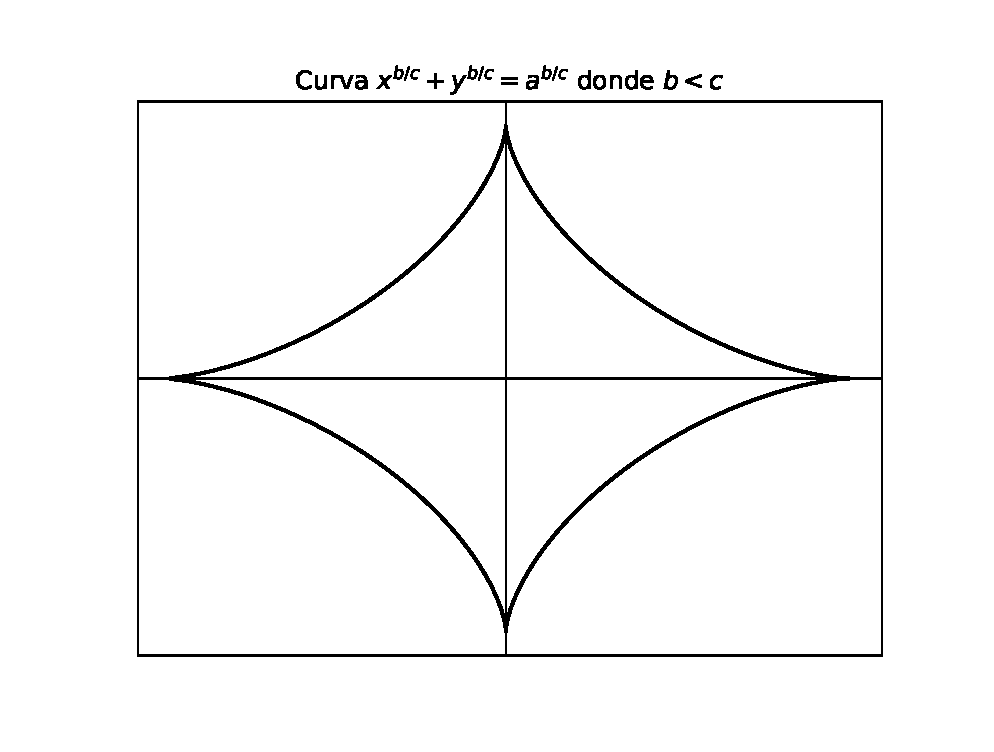
\includegraphics[scale=0.5]{Imagenes/plot_curva_estrella_01.eps}
    \caption{Estrella con cuatro picos cóncavos.}
    \label{fig:figura_curva_estrella}
\end{figure}
\end{frame}
\begin{frame}
\frametitle{Enunciado del problema}
Calcula el área dentro de la curva (ec. \ref{eq:ecuacion_curva_estrella}) en términos de la función Gamma cuando el exponente $b/c$ es $2/3$.
\end{frame}
\begin{frame}
\frametitle{Antes de la Solución}
Antes de resolver el problema, nos conviene observar que la familia de curvas representadas por la ecuación (\ref{eq:ecuacion_curva_estrella}) tiene como uno de sus miembros la conocida estrella de cuatro puntas o \emph{astroide}\footnote{También se le conoce como tetracúspide, cubocicloide, o paraciclo.}:
\begin{align*}
x^{2/3} + y^{2/3} = a^{2/3}
\end{align*}
\end{frame}
\begin{frame}
\frametitle{Antes de la Solución}
De hecho, siempre que $b < c$, se tiene una estrella cóncava con cuatro puntas afiladas (cúspides).
\\
\bigskip
Por otro lado, cuando $b > c$, la curva es convexa; y cuando $c = 1$ y $b$ es un entero par grande, la curva es casi un cuadrado.
\end{frame}
\begin{frame}
\frametitle{Antes de la Solución}
En cualquier caso, la curva es simétrica en ambos ejes de coordenadas, de modo que podemos \emph{calcular solo la parte del área que está en el primer cuadrante} y multiplicaremos el resultado por $4$ para obtener el área completa dentro de la curva.
\end{frame}
\begin{frame}
\frametitle{Antes de la solución}
\begin{figure}[H]
    \centering
    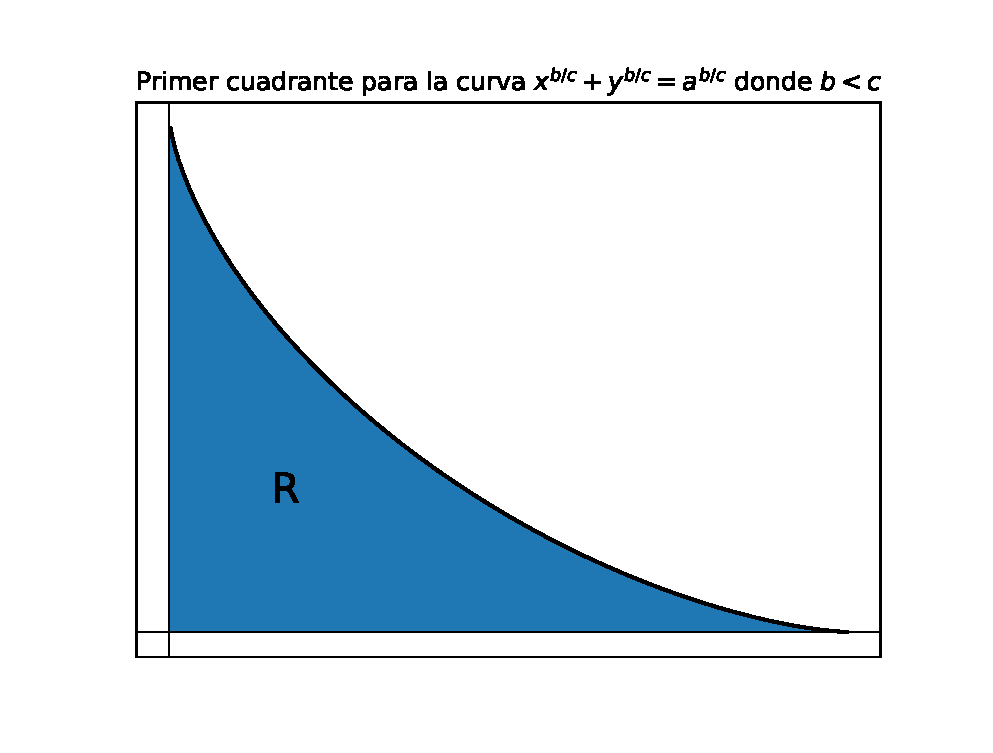
\includegraphics[scale=0.5]{Imagenes/plot_curva_estrella_02.eps}
    \caption{Cuadrante de trabajo para calcular el área.}
    \label{fig:figura_curva_estrella_cuadrante}
\end{figure}
\end{frame}
\begin{frame}
\frametitle{Solución general}
Obtendremos inicialmente una solución general para valores $a$, $b$ y $c$, posteriormente calcularemos la solución particular con los valores que nos da el enunciado: $b = 2$ y $c = 3$.
\end{frame}
\begin{frame}
\frametitle{Solución general}
Tenemos entonces que:
\pause
\begin{align*}
\text{Área = } 4 \scalebox{2}{$\iint$}_{R} \dd{A}
\end{align*}
donde $R$ representa la región en el primer cuadrante rodeado por la curva y los ejes.
\end{frame}
\begin{frame}
\frametitle{Solución a la integral}
Hacemos la doble integral a una integral equivalente con límites:
\pause
\begin{align*}
A = 4 \scaleint{6ex}_{\bs 0}^{a} \dd{x} \, \scaleint{6ex}_{\bs 0}^{\left( a^{b/c} - x^{b/c} \right)^{c/b}} \dd{y}
\end{align*}
\end{frame}
\begin{frame}
\frametitle{Cambio de variable para $y$}
Para evaluar la integral en $y$, hacemos el siguiente cambio de variable:
\pause
\begin{align*}
y = a \, v^{\frac{c}{b}} \hspace{1cm} \Longrightarrow \hspace{1cm} \dd{y} = a \, \left( \dfrac{c}{b} \right) \, v^{\frac{c}{b} - 1} \dd{v}
\end{align*}
\end{frame}
\begin{frame}
\frametitle{Cambio de variable para $x$}
Mientras estamos en eso, también podemos hacer el mismo tipo de cambio en la variable para $x$:
\pause 
\begin{align*}
x = a \, u^{\frac{c}{b}} \hspace{1cm} \Longrightarrow \hspace{1cm} \dd{x} = a \, \left( \dfrac{c}{b} \right) \, u^{\frac{c}{b} - 1} \dd{u}
\end{align*}
\end{frame}
\begin{frame}
\frametitle{Nuevos límites de integración}
Al realizar los cambios de variables, corresponde entonces también realizar el cambio en los límites de integración, por lo tanto:
\pause 
\begin{align*}
A = \dfrac{4 \, a^{2} \, c^{2}}{b^{2}} \, \scaleint{6ex}_{\bs 0}^{1} u^{\frac{c}{b} - 1} \dd{u} \, \scaleint{6ex}_{\bs 0}^{1-u} v^{\frac{c}{b} - 1} \dd{v}
\end{align*}
\end{frame}
\begin{frame}
\frametitle{Integrando con respecto a $v$}
Al realizar la integración con respecto a $v$, tenemos:
\pause 
\begin{align*}
A = 4 \, a^{2} \, \left( \dfrac{c}{b} \right) \, \scaleint{6ex}_{\bs 0}^{1} u^{\frac{c}{b} - 1} (1 - u)^{c/b} \dd{u}
\end{align*}
\pause
Recordando que la función Beta se define como:
\pause 
\begin{align*}
B(x, y) = \scaleint{6ex}_{\bs 0}^{1} t^{x-1} (1 - t)^{y-1} \dd{t} \hspace{1cm} x > 0, y > 0
\end{align*}
\end{frame}
\begin{frame}
\frametitle{Resultado parcial}
Encontramos una buena utilidad para las funciones que involucran integrales, ya que el cálculo de éstas se simplifica mucho.
\\
\bigskip
\pause
Entonces la integral anterior en la expresión para el área $A$, es la integral Beta, por tanto:
\end{frame}
\begin{frame}
\frametitle{Resultado parcial}
Tenemos que:
\pause
\begin{align*}
A = 4 \, \left( \dfrac{c}{b} \right) \, a^{2} \, B \left( \dfrac{c}{b}, \dfrac{c}{b} + 1 \right)
\end{align*}
\pause
Para resolver la expresión en términos mucho más sencillos, debemos de ocupar las propiedades e identidades para las funciones Gamma y Beta, como veremos a continuación:
\end{frame}
\begin{frame}
\frametitle{Ocupando propiedades}
Conocemos una expresión que relaciona la función Beta con la Gamma, entonces tendremos que:
\pause 
\begin{align*}
A = 4 \, \left( \dfrac{c}{b} \right) \, a^{2} \, \left[ \dfrac{\mathlarger{\Gamma} \left( \dfrac{c}{b} \right) \, \mathlarger{\Gamma} \left( \dfrac{c}{b} + 1 \right)}{\mathlarger{\Gamma} \left( \dfrac{2 \, c}{b} + 1 \right)} \right]
\end{align*}
\end{frame}
\begin{frame}
\frametitle{Ocupando propiedades}
Seguimos ocupando las identidades de la función Gamma:
\pause 
\begin{align*}
\mathlarger{\Gamma} \left( \dfrac{c}{b} + 1 \right) &= \dfrac{c}{b} \, \mathlarger{\Gamma} \left( \dfrac{c}{b} \right) \\[1em]
\mathlarger{\Gamma} \left( \dfrac{2 \, c}{b} + 1 \right) &= \dfrac{2 \, c}{b} \, \mathlarger{\Gamma} \left( \dfrac{2 \, c}{b} \right)
\end{align*}
\end{frame}
\begin{frame}
\frametitle{Solución general}
La solución general para el área contenida en el astroide es:
\pause
\begin{align*}
A = \dfrac{\mathlarger{\Gamma} \left( \dfrac{c}{b} \right) \, \mathlarger{\Gamma} \left( \dfrac{c}{b} \right)}{\mathlarger{\Gamma} \left( \dfrac{2 \, c}{b} \right)} \, \left( \dfrac{2 \, c \, a^{2}}{b} \right)
\end{align*}
\pause
Por lo que tenemos una expresión más sencilla que involucra la evaluación de la función Gamma, para cualesquiera valores de $b$ y $c$.
\end{frame}
\begin{frame}
\frametitle{Solución particular}
El área del astroide cuando $b = 2$ y $c = 3$ es:
\pause
\begin{align*}
A &= \dfrac{\mathlarger{\Gamma} \left( \dfrac{3}{2} \right) \, \mathlarger{\Gamma} \left( \dfrac{3}{2} \right)}{\mathlarger{\Gamma} (3)} \, (2) \left( \dfrac{3}{2} \right) \, a^{2} \\[1em]
&= \dfrac{3 \, a^{2} \, \pi}{8} \qed
\end{align*}
\end{frame}

\end{document}